%% LaTeX2e class for student theses
%% sections/content.tex
%% 
%% Karlsruhe Institute of Technology
%% Institute for Program Structures and Data Organization
%% Chair for Software Design and Quality (SDQ)
%%
%% Dr.-Ing. Erik Burger
%% burger@kit.edu
%%
%% Version 1.3.6, 2022-09-28

\chapter{Background}
\label{ch:Background}

In this chapter we will give an overview of the background knowledge that is needed to understand the following chapters. The topic
of this thesis is at the intersection of the fields of Active Learning, Continual Learning and Model Stealing and therefore we will
give an introduction to each of these fields. 

\section{Active Learning}
\label{sec:ActiveLearning}

%TODO: Hier learner-Beschreibung anpassen und ggf. Batch Active Learning einführen (Warum nötig? Für NNs)
% Representation-based active learning und diversity-based active learning sind quasi gleich, das noch erwähnen
Active Learning is a subfield of Machine Learning that focuses on the problem of how to select the most informative data points to label.
Research in Active Learning is motivated by the fact that data acquisition is often easy because it can be automated whereas labeling is
difficult and time-consuming. Therefore, the goal of research in Active Learning is to develop methods which maximize model performance
with minimal amount of labeled data. A typical Active Learning scenario comprises a learner, an oracle, unlabeled data and labeled data.
The learner is the actual algorithm which selects which data points to label by the oracle. Let $I$ be the instance space (i.e. the set
of all possible data points) and $L$ be the label space (i.e. the set of all possible labels). The oracle $O$ can be seen as the function
\begin{equation}
    O: I \rightarrow L, x \mapsto y(x)
\end{equation}
where $y(x)$ is the true label of the data point $x$, often just referred to as $y$. The unlabeled data $U$ is a subset of $I$ just as the set
of labeled data $L$. At the beginning there are no labeled data points. Often a few labeled data points are randomly sampled from $U$ and labeled
by the oracle to initialize the learning process. A detailed overview on research activities within the Active Learning Domain is presented in
\cite{settles2009active}. Note however that more recent works are not contained in this literature survey because it was last updated in 2009.
In general, Active Learning methods can be divided into three categories:
\begin{itemize}
    \item \textbf{Query Synthesis Active Learning}
    \item \textbf{Pool-based Active Learning}
    \item \textbf{Stream-based Active Learning}
\end{itemize}
The taxonomy mentioned above is composed in a data-centric way. While researchers generally agree on the taxonomy mentioned above,
it is important to note that the effectiveness of an active learning strategy also depends on the type of Machine Learning Model that is used
(e.g. (Convolutional) Neural Networks, Support Vector Machines, etc.) and the type of data that is used (e.g. images or text).
For example, the pool-based Active Learning strategy CoreSet \cite{sener2017active} was specifically designed for CNNs.

\subsection{Query Synthesis Active Learning}
\label{sec:QuerySynthesisActiveLearning}
Query Synthesis Active Learning, also known as Membership Query Synthesis Active Learning, was among the first active learning scenarios
that were proposed \cite{angluin1988queries}. The idea behind this approach is to synthesize data points from the input space, rather than
to sample real data points. Nowadays, this is done by training a generative model (e.g a Generative Adversarial Network) \cite{zhu2017generative}
which learns the distribution of unlabeled data. However, earlier works relied on statistical models such as Gaussian Mixture Models 
\cite{cohn1996active}. The generated queries are then labeled by the oracle and can be used to train the Machine Learning Model. Note that
Query Synthesis is not limited to classification tasks. For example, \cite{cohn1996active} proposed a method to predict the absolute coordinates
of a robot hand when given the joint angles of its mechanical arms as inputs. When the oracle is a human annotator, Query Synthesis Active Learning
researchers have encountered problems in labeling them. Because the generated queries do not show any class-discriminative features, human annotators
struggled to assign any class to them in the survey of \cite{baum1992query}.

% TODO: Hier ein Bild wie QS Active Learning funktioniert einfügen

\subsection{Pool-based Active Learning}
\label{sec:PoolBasedActiveLearning}
Pool-based Active Learning is the most widely studied and used type of Active Learning. The idea behind pool-based Active Learning approaches
is to iteratively select the most informative data points from the current unlabeled pool, query the oracle for their labels and add them to the
labeled pool. Next, the ML model is trained on the current labeled pool. This process is repeated until the query budget is exhausted. A more detailed
explanation can be found in \ref{alg:PoolBasedActiveLearning}. More formally, the pool-based Active Learning problem can be defined as:
\begin{equation}
    \min_{s^1 \subseteq U: |s^1| \leq b} E_{x,y \sim P_{(X,Y)}}[l(x,y;L \cup b)]
\end{equation}
In other words, a pool-based Active Learning algorithm aims to select the points that minimize the expected loss of the model on the labeled pool when
being added to it. As can be seen from  \ref{alg:PoolBasedActiveLearning} the structure across Pool-based Active Learning strategies is very similar.
The main difference between them is the informative measure, i.e. the criterion with which they select which data points to label next. Within the 
Pool-based Active Learning category, there are two subcategories: \textbf{Uncertainty-based} sampling and \textbf{Diversity-based} sampling. 
Uncertainty-based sampling strategies select the data points that the model is most uncertain about. Diversity-based sampling strategies on the other
hand aim to select data points that best represent the data distribution in the unlabeled pool. All the active learning strategies that we will use
are pool-based Active Learning Strategies, stemming both from the Uncertainty-based and Diversity-based subcategories.

\begin{algorithm}
    \caption{Pool-based Active Learning} \label{alg:PoolBasedActiveLearning}
    \begin{algorithmic}[1]
        \Require Unlabeled data $U$,Labeled data $L = \emptyset$:, Oracle $O$, Model $M$, budget $B$
        \State Select $k$ data points from $U$ at random, obtain labels by querying $O$ and set $L=\{x_1,\ldots,x_1\}$
        and $U = U \setminus \{x_1,\ldots,x_1\}$ \Comment{Initialization}
        \State Train $M$ on initial labeled set $L$
        \While{label budget $B$ not exhausted}
            \State Select $l$ data points from $U$ predicted to be the most informative by the Active Learning strategy
            \State Obtain labels by querying $O$ for $x_i,\ldots,x_l$
            \State Set $L= L \cup \{x_i,\ldots,x_l\}$ and $U = U \setminus \{x_i,\ldots,x_l\}$
            \State Train $M$ on labeled set $L$
        \EndWhile
    \end{algorithmic}
\end{algorithm}

\subsection{Stream-based Active Learning}
\label{sec:StreamBasedActiveLearning}
Stream-based Active Learning is closer to Pool-based Active Learning than Query Synthesis Active Learning. It was first introduced by Cohn et al. 
\cite{cohn1994improving}. The main difference between Stream-based Active Learning and Pool-based Active Learning is that data arrives sequentially
instead of having a batch of data points at once. In the stream-based Active Learning scenario, the learner draws a data point from the data source
one at a time. For each data point, the learner can then decide to query the oracle for its label or to discard it. The decision whether to label a
data point can either be made on the basis of its informativeness \cite{dagan1995committee} or its location within the instance space \cite{cohn1994improving}.
In the latter case the learner would label the data point if it is located in a region of the instance space that the learner is not confident about.

\section{Continual Learning}
\label{sec:ContinualLearning}
Continual Learning is a subfield of Machine Learning that aims to solve the problem of catastrophic forgetting. To elaborate further on this problem,
it is important to remember that most machine learning services are deployed in an environment where constant changes occur. To adapt to this, it is
necessary for Machine Learning Models to learn continually, i.e. to learn new tasks without forgetting the knowledge they have acquired in the past.
This is a common case for humans. For example, if a child has once learned to walk, it does not forget how to walk when it learns to ride a bike.
In contrast to human behavior, the performance of Machine Learning Models on old tasks rapidly decreases when they are trained on new tasks. This phenomenon
is known as \enquote{Catastrophic Forgetting} and was already discovered in the early days of Machine Learning research \cite{mccloskey1989catastrophic}.
In more general terms, research in Continual Learning is looking not only to alleviate Catastrophic Forgetting, but to solve the 
\enquote{stabiliy / plasticity dilemma} \cite{carpenter1988art}. The stability / plasticity dilemma refers to the fact that Machine Learning Models
should ideally be stable enough to retain their performance on old tasks while simultaneously being plastic enough to adapt to new tasks. This is a dilemma
because both properties are designed even though they are in conflict with each other. In practice, Machine Learning Models are rather plastic than stable.
This is especially true for Deep Neural Networks, but generally for all Machine Learning Models that are trained by greedily updating their parameters using
gradient descent \cite{mundt2020wholistic}. \\
Continual Learning is mainly used in scenarios where new tasks arrive over time or where the data distribution changes over time. Despite being useful
in these classic scenarios, Continual Learning approaches can also be used in cases where the data cannot be stored for legal reasons or due to memory
constraints, i.e. when the normal batch learning approach with a large training set cannot be applied. 


\subsection{Continual Learning Scenarios}
\label{sec:ContinualLearningScenarios}
Continual Learning is a rapidly evolving research field and terminology and taxonomy are still being established. Among the most important factors to distinguish
is the way in which new tasks arrive. In the following, we will introduce the three typical Continual Learning Scenarios as presented in \cite{van2022three}. 

\subsubsection{Task-Incremental Continual Learning}
\label{sec:TaskIncrementalContinualLearning}
%TODO: Add a figure that shows the difference between the three scenarios. For Task-Incremental learning mention tuple with task id.
In the Task-Incremental setting, a model is informed about which task it will be trained on or which task the data whose label it is supposed to predict belongs to.
The task-information is supplied via a task identifier which is usually an integer. Because the model does not have to infer the task which it is supposed to predict
or learn, it is possible to have task-specific components in the model. For neural networks, this means that there is one output layer per task and for each task the
respective output layer is used while all other layers are shared between all tasks. These classifiers are also known as \enquote{multi-head} classifiers \cite{van2018generative}.
An example would be the following: The first task is to classify images of cats and dogs. The second task is to classify cows and sheep. The model would have one output layer 
used to classify cats and dogs and a second output layer to classify cows and sheep. When training for the first task, only the first output layer is used. When the second task
arrives the model is retrained with the second output layer.  The mapping that is learned is 
\begin{equation}
    f: X \times T \rightarrow Y
\end{equation}
Where $X = \mathbb{R}^{N x N x C}$ is the input space (i.e. all possible input images of size $N x N$ with $C$ channels), $T = \{1,2,\ldots\}$ is the task space (i.e. all possible
tasks that the model can be trained on) and $Y = \mathbb{Z}_{k}$ is the label space with $k$ being the number of possible classes.
% Figure with decision tree for the continual learning scenarios like in https://www.nature.com/articles/s42256-022-00568-3
\subsubsection{Domain-Incremental Continual Learning}
\label{sec:DomainIncrementalContinualLearning}
In the Domain-Incremental setting, task identities are not given during evaluation. Since the underlying task does not change, this is also not necessary. While the structure of the task
stays the same it is rather the distribution of the data that changes. An example of Domain-Incremental Continual Learning would be the classification of digits between 0 and 9 (such as
those in the MNIST dataset) where the digits for one subtask are green and blue for the other. The mapping that is learned is 
\begin{equation}
    f: X \rightarrow Y
\end{equation}
Where $X = \mathbb{R}^{N x N x C}$ is the input space (i.e. all possible input images of size $N x N$ with $C$ channels), and $Y = \mathbb{Z}_{k}$ is the label space with $k$ being the
number of possible classes.

\subsubsection{Class-Incremental Continual Learning}
\label{sec:ClassIncrementalContinualLearning}
Class-Incremental Continual Learning is the most challenging scenario. Like in the Domain-Incremental setting, task identities are not provided at evaluation time, however, this time they
need to be inferred by the model. In this scenario, a classifier would be incrementally exposed to multiple tasks which contain different classes. An example would be again the classification
of digits between 0 and 9, where this time each task contains a disjoint subset of digits. The classifier would be trained on the first task, containing the digits 0 and 1, the second task,
containing the digits 2 and 3 and so on. During evaluation, the classifier would not only have to classify the digits correctly, but also to infer which task they belong to. The mapping that
is learned is 
\begin{equation}
    f: X \rightarrow Y \times T
\end{equation}
Where $X = \mathbb{R}^{N x N x C}$ is the input space (i.e. all possible input images of size $N x N$ with $C$ channels), $T = \{1,2,\ldots\}$ is the task space (i.e. all possible
tasks that the model can be trained on) and $Y = \mathbb{Z}_{k}$ is the label space with $k$ being the number of possible classes.

\subsection{Continual Learning Approaches}
\label{sec:ContinualLearningApproaches}
The Continual Learning approaches which have been proposed so far can be grouped into three categories according to, \cite{parisi2019continual} \cite{mundt2020wholistic} and \cite{zenke2017continual}.
Parisi et al. \cite{parisi2019continual} propose to group Continual Learning approaches into \textbf{regularization}, \textbf{rehearsal} and \textbf{architectural} approaches whereas Zenke et al.
\cite{zenke2017continual} group Continual Learning approaches into \textbf{architectural},\textbf{functional} and \textbf{structural} approaches. In the following, we will stick to the
categorization proposed by Parisi et al. because it is broader and fully encompasses the categorization by Zenke et al. Furthermore, Parisi et al.'s classification has been adopted by
recent continual learning reviews \cite{mundt2020wholistic}.

\subsubsection{Regularization Approaches}
\label{sec:RegularizationApproaches}
Regularization-based approaches to Continual Learning aim to prevent the forgetting of previous tasks by adding a regularization
term to the model's loss function. The regularization term is used as a proxy for how much the performance of the model on previous
tasks will decrease, i.e. a high regularization term indicates that the model will perform poorly on the old tasks with the current
weights and a low regularization term indicates that the model has not lost much knowledge of the old tasks. The way the
regularization term is computed can further be divided into two groups. There are \textbf{structural} approaches which regularize
based on weight changes to the model and there are \textbf{functional} approaches which regularize based on the output of the model.
Notable examples of structural approaches include Elastic Weight Consolidation (EWC) \cite{kirkpatrick2017overcoming},Memory Aware
Synapses (MAS) \cite{aljundi2018memory}, Incremental Moment Matching (IMM) \cite{lee2017overcoming} as well as Asymmetric Loss
Approximation by Single-Side Overestimation (ALASSO) \cite{park2019continual} which is an extension of Synaptic Intelligence (SI)
\cite{zenke2017continual}. All the structural regularization approaches will be covered in more detail in the section on
\hyperref[sec:Related_work:Continual_Learning:Experiments]{the continual learning approaches used in the experiments}. \\
Functional regularization approaches are inspired by knowledge distillation \cite{hinton2015distilling}. They add a distillation
loss to the objective function which is computed based on the prediction of a data sample stored for future use. These data samples
are called soft targets. Li et al. \cite{li2017learning} compute the distillation loss by using the output of the newly arrived task
given by the model trained on the old tasks. The distillation loss they introduce aims to retain the prediction of the old model on
the new task even if the prediction itself may be inaccurate. The approach of Rannen et al. \cite{rannen2017encoder}, called Encoder
Based Lifelong Learning (EBLL) is based on the approach of Li et al., however in EBLL the distillation loss is computed based on
autoencoder reconstructions of old tasks.

\subsubsection{Rehearsal Approaches}
\label{sec:RehearsalApproaches}
Rehearsal approaches to Continual Learning aim to prevent catastrophic forgetting by fitting a model's parameters to the distribution
of an incoming task and all previous tasks simultaneously. Within Rehearsal approaches it is important to remember the trade-off between
model performance and computational cost. In general, the more data from previous tasks is used to train the model, the better the accuracy is. 
However, in order to train on more data, the data has to be stored and fed into the training process which is costly in terms of memory and This can either be done by replaying stored data from previous tasks or by
retraining on generated data drawn from the distribution of previous tasks. Continual Learning Methods that rely on the former idea are
categorized as \textbf{exemplar rehearsal} approaches while those that rely on the latter idea are categorized as \textbf{generative replay}
approaches. \\
Exemplar Rehearsal Techniques store data from previous tasks in a so-called \enquote{Replay Buffer} which data is sampled



\subsubsection{Architectural Approaches}
\label{sec:ArchitecturalApproaches}

\section{Model Stealing}
\label{sec:ModelStealing}
% TODO: Add figure with model stealing process
% Model Stealing notes: 
% Taxonomy provided by Jagielski et al. based on attacker's goal 
% Four types of attacks presented by He et al.: model extraction, model inversion, model poisoning and adversarial attack.
% Model extraction is a subfield of adversarial machine learning.
% Look at section 4.3 of Oliynyk et al. paper for taxonomy of adversarial ml.
% Mention some notation as in Olinyk et al. paper in section 5.1.
% Metrics to measure attack in 5.4 of Olinyk et al. paper.
% Have a look at Fig3 of Olinyk et al. paper and use it to tell which attacks we use (e.g. NNPD, Computer Vision, etc.)
% Based on Olinyk et al., our approach falls into the consistency category of section 6.1
% Model Stealing defenses are either used for attack detection or attack prevention.
% TODO: Add connection to Knowledge distillation as mentioned in Related Work section of ActiveThief paper.
With the advent of Machine Learning as a Service (MLaaS), an increasing amount of machine learning models are being exposed to the public via 
prediction APIs. The idea of these prediction APIs is that a user can request a prediction from a model by sending a request containing an unlabeled data
point to the API. The response to the request is then the prediction of the model for the data point. Prediction APIs are monetized by charging the user
on a pay-per-query principle. That means that each request has a fixed price for each query which is usually subtracted from his or her account balance on
a monthly basis. Providing public access to a machine learning model is a win-win situation because the model developer is compensated for his or her efforts
on gathering and labeling appropriate training data, choosing a proper model architecture, training the model and fine-tuning its hyperparameters while the user
of the prediction API can benefit from the model's predictions without having to train the model himself or herself. \\
Since the developed model is the intellectual property of the model developer, it is important that only the model's predictions are exposed to the public and
not the model (i.e. its architecture and the model weights)itself. However, in the last years numerous research papers have been published which demonstrate how
several features of a machine learning model can be extracted, i.e. its functionality \cite{tramer2016stealing}, its architecture \cite{oh2019towards} and its
training data \cite{shokri2017membership}. This newly created field of research is called \textbf{Model Stealing} or \textbf{Model Extraction}, and it is a subfield
of \textbf{Adversarial Machine Learning} according to Oliynyk et al. \cite{oliynyk2022know}. Because Model Extraction attacks are so effective, further research works
concerning model stealing defense mechanisms have been published. In the following we will use the taxonomy provided by Oliynyk et al. (see Figure 
\ref{fig:ModelStealing:Taxonomy}) \cite{oliynyk2022know} as a basis for our categorization of Model Stealing attacks and defenses. \\

\subsection{Terminology}
\label{sec:ModelStealing:Terminology}
Since Model Stealing is a rather new field it comes with numerous terms that are not commonly used in other fields of machine learning and others that are used 
synonymously. In order to avoid confusion, we will define and explain the terms we use in this section and. \\
\textbf{Model Stealing Attack}: The process of maliciously querying a machine learning model in order to extract some or all of the model's features, such as its
architecture, its weights or its training data. Model Stealing Attacks are also known as Model Extraction Attacks or Model Inference Attacks among others. \\
\textbf{Target Model}: The model that is queried via the prediction API and whose features the attacker aims to extract. The target model has also been referred to 
as Oracle, Victim Model or Secret Model. \\
\textbf{Substitute Model}: The model that is used by the attacker to extract the target model's features. Synonyms for Substitute Model are Adversarial Classifier,
Knockoff Model or Inferred Model. \cite{orekondy2019knockoff} have demonstrated that is favorable to choose a rather complex model architecture which is in line with 
our findings.\\
\textbf{Target Model Dataset}: The dataset that the target model has been trained on. The term Target Model Dataset has not been used in the literature before (to 
the best of our knowledge), but we choose this term over the synonymous term Secret Dataset because we believe it is more expressive. During Model Stealing Attacks,
the attacker does not have access to the target model's dataset, i.e. it is kept secret. For research purposes however, a test set of the Target Model Dataset is
used to evaluate the performance of the Substitute Model. \\
\textbf{Thief Dataset}: The dataset that is used by the attacker to train the Substitute Model. The Thief Dataset is also known as Fake dataset, Attacker Set or 
Transfer Set. When constructing the Thief Dataset, the attacker can either use \textbf{Natural Non-Problem Domain} (NNPD) or \textbf{Synthetic Non-Problem Domain} (SNPD)
data. NNPD data is data that is collected from the real world but does not (knowingly) overlap with the Target Model Dataset whereas SNPD data is artificially created,
usually by drawing from a given distribution such as a multidimensional Uniform Distribution \cite{pal2020activethief}. Empirical observations show that using NNPD data
yields significantly better results than using SNPD data. Even when using NNPD data, significant differences between different datasets have been observed 
\cite{pal2020activethief}. In general, it is wise to choose a dataset that is as diverse as possible. Regardless of using SNPD or NNPD data, the adversary should keep the
dimensions of the Target Model Dataset, i.e. image size and especially the number of channels for image datasets, in mind and adapt the Thief Dataset accordingly. \\
\textbf{Agreement}: The relative agreement between the predictions of the Substitute Model and the Target Model. The agreement is computed on a test set of the Target 
Model dataset, meaning that it is not accessible by the attacker. The agreement is also known as Extraction accuracy, label prediction match or similarity. More formally,
the agreement between Target Model $f$ and Substitute Model $\tilde{f}$ is defined as follows:
\begin{equation}
    Agreement(f,\tilde{f}) = \frac{1}{|X_{tm}^{test}|} \sum_{x \in X_{tm}^{test}} \mathds{1}(f(x) = \tilde{f}(x))
\end{equation}




\subsection{Model Stealing Attacks}
\label{sec:ModelStealing:Attacks}
Model Stealing attacks can be performed in a variety of ways. The methodology with which such an attack is executed depends on the goal of the attacker. If the attacker
aims to extract training hyperparameters, then he or she can use an equation-solving approach \cite{wang2018stealing} or train a meta-model to predict the hyperparameters
\cite{oh2019towards}. The meta-model approach proposed by Oh et al. can also be used to extract the model architecture. This is the only approach that does not rely on either
software or hardware access to the target model. Other approaches, such as the one proposed by Yan et al. \cite{yan2020cache}, make use of side-channel attacks to extract
the architecture of the target model and therefore require software or hardware access to the target model. \\
Apart from extracting training hyperparameters or model architecture, the attacker might also be interested in the target model's weights, also called learned parameters. This
is especially the case if the model architecture and/or training hyperparameters are already known. These can be known because they are not kept secret but also by using the 
aforementioned attacks to extract them. It is important to note here that different Model Stealing Attacks should not be seen as mutually exclusive but rather as a toolkit that,
while often used individually, can be combined to extract a wholistic view of the target model. So far, attacks have been proposed to extract the weights of a binary classifier
\cite{lowd2005adversarial},logistic regression \cite{tramer2016stealing}, simple Neural Networks \cite{tramer2016stealing} and support vector regression \cite{reith2019efficiently}. \\
Many attackers are not interested in specific model features, such as architecture or (hyper-) parameters but rather in reproducing the target model's \textit{functionality}, i.e.
its ability to predict a label for a given input. When stealing model functionality, attackers either aim to maximize the accuracy of the substitute model on the target model's
test set or maximize the agreement between the predictions of the substitute model and the target model. While Oliynyk et al. list these as separate attacks, we believe that it is
rather a matter of what the optimization objective is. Regardless of whether the attacker aims to maximize the accuracy or agreement, the attacker has to train a substitute model
and choose an appropriate thief dataset. Empirical observation have shown that choosing a rather complex model architecture for the substitute model yields better results if the
model architecture is unknown whereas choosing a model architecture that is a similar to the target model's architecture as possible yields better results if the model architecture
is known \cite{orekondy2019knockoff} \cite{pal2020activethief}. \\

\begin{figure} [ht]
  \centering
  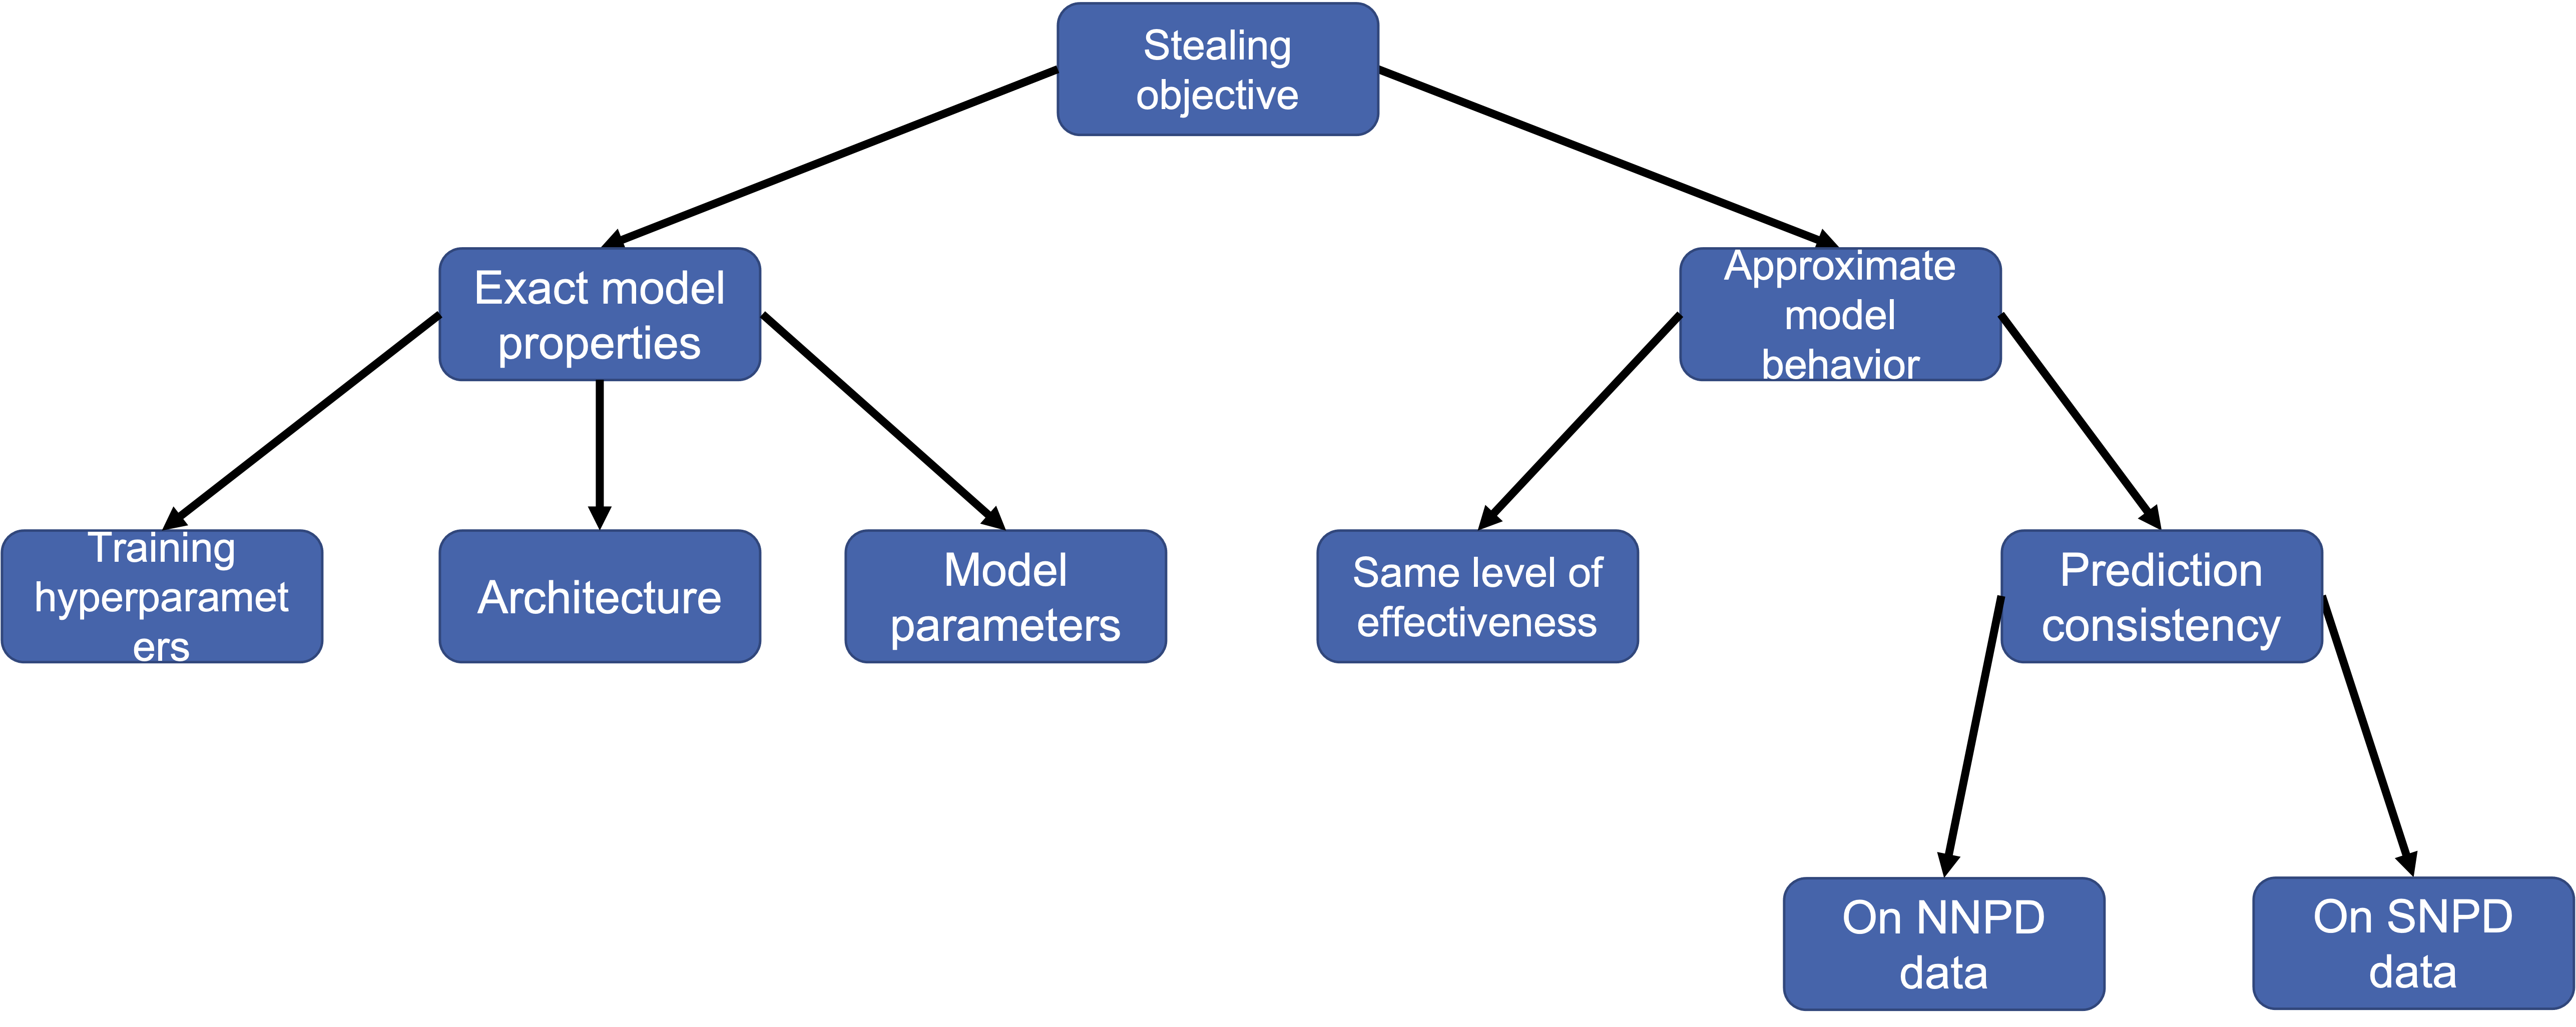
\includegraphics[width=.9\linewidth]{images/MS_Taxonomy.png}
  \caption[Model Stealing Taxonomy]{Taxonomy of Model Stealing Attacks by \cite{oliynyk2022know}}
  \label{fig:ModelStealing:Taxonomy}
\end{figure}


\subsection{Model Stealing Defenses}
\label{sec:ModelStealing:Defenses}
Because of the detrimental effect of Model Stealing Attacks, many defenses have been proposed to protect against them. Defenses can be categorized into proactive and
reactive defenses. While proactive defenses actively aim to prevent or at least complicate Model Stealing Attacks, reactive approaches purely aim to detect them.

\subsubsection{Reactive Model Stealing Defenses (Detection)}
\label{sec:ModelStealing:Defenses:Detection}
Reactive Model Stealing Defenses solely aim to detect Model Stealing Attacks, not prevent them from happening. So far there exist Model Stealing Detection Approaches which
rely either on Watermarking or on Monitoring. Watermarking is a way to prove ownership of a machine learning model. This is usually achieved by \enquote{hiding} information
in the model which can only be restored by the original owner. A watermark can be a predefined prediction value for outlier samples which are unlikely to be part of the thief
dataset. Watermarking can be applied during training \cite{zhang2018protecting} or afterwards \cite{szyller2021dawn}. Monitoring is a way to detect Model Stealing Attacks by
investigating the queries that a user made to the target model. Kesarwani et al. \cite{kesarwani2018model} proposed a method that estimates the relative amount of the data space that a user has
covered with his queries. Based on this metric they can infer the status of a possible extraction attack. Another approach named PRADA \cite{juuti2019prada} analyses the distribution of the
samples that a user has queried so far. They assume that the distance between queries of a benign user follows a normal distribution and any user whose query distances are not normally
distributed is considered to be an attacker. \\

\begin{figure} [ht]
    \centering
    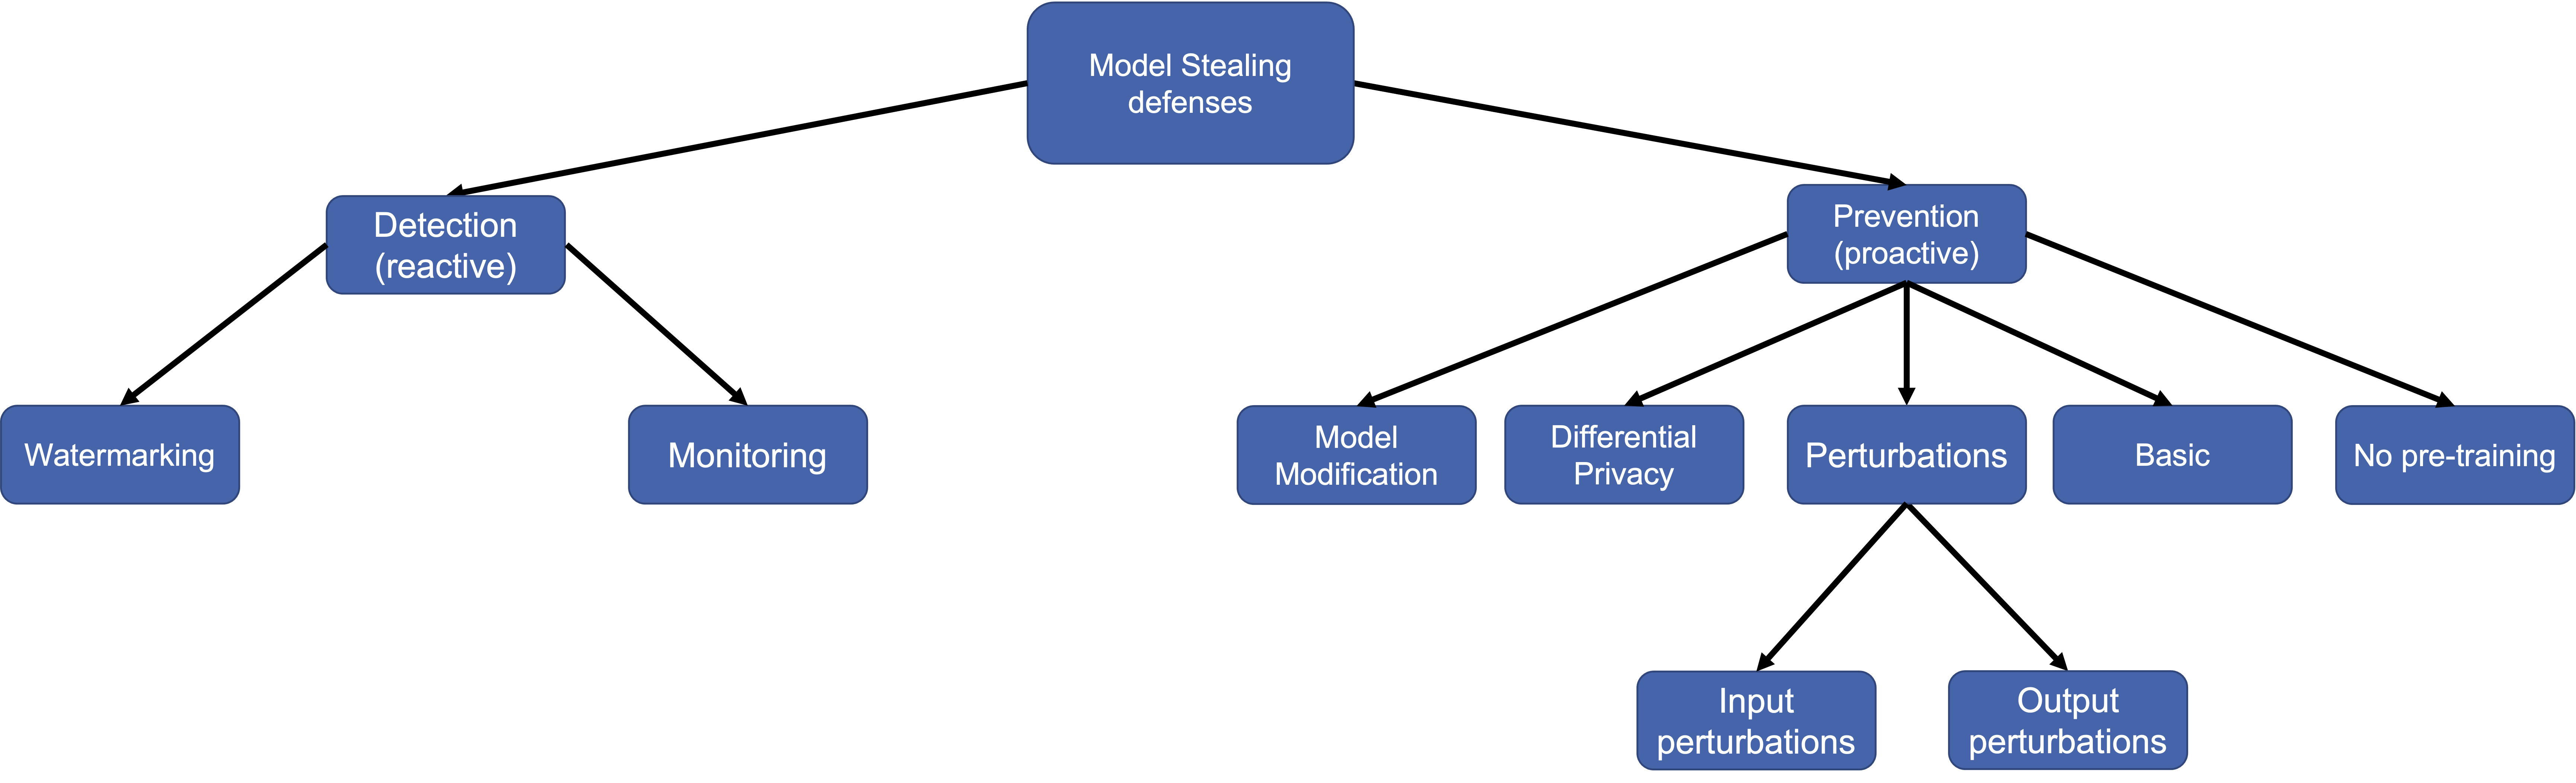
\includegraphics[width=.9\linewidth]{images/MS_defenses_Taxonomy.png}
    \caption[Model Stealing Defenses Taxonomy]{Taxonomy of Model Stealing Defenses by \cite{oliynyk2022know}}
    \label{fig:ModelStealingDefenses:Taxonomy}
  \end{figure}

\subsubsection{Proactive Model Stealing Defenses (Prevention)}
\label{sec:ModelStealing:Defenses:Prevention}
Proactive Model Stealing Defenses aim to complicate or prevent Model Stealing Attacks from happening. It is important to note that the success of a Model Stealing attack is not binary,
compared to breaking into a house for example. Model Stealing Attacks will always be successful to some degree, but their success mainly depends on the accuracy that the substitute model
can achieve (or the achieved model agreement in case the attacker tries to optimize for that). So the quality of a Proactive Model Stealing Defense should be measured by how much it can 
decrease the accuracy of the substitute model compared to a Model Stealing Attack with no defense. A key challenge in developing Proactive Model Stealing Defenses is that, on one hand,
it should be complicated to extract the target model while on the other hand the user experience of benign users should not be affected. \\
Early on, a few basic approaches against Model Stealing Attacks were proposed. These include training several models and randomly choosing the output of one of them 
\cite{alabdulmohsin2014adding}. An even simpler albeit effective approach is to output only the predicted label instead of the vector of output probabilities \cite{tramer2016stealing}.
A downside to this is that a benign user loses a lot of information about the output and the model is less interpretable. Another approach that is similar in complexity is to renounce
using pre-trained models \cite{atli2020extraction} and instead train the target model from scratch. \\
In order to prevent Model Stealing Attacks, researchers have proposed to use data perturbation. One can either choose to perturb the data that is fed to the target model or its prediction.
Input perturbation can for example be performed by adding noise to unimportant pixels determined via Gradient Class Activation Maps \cite{guiga2020neural}. To perform output perturbation,
the developer of the target model can either use Maximizing Angular Deviation (MAD) \cite{orekondy2019prediction} or flip a few labels to obfuscate the model's decision boundary
\cite{shi2017evasion}. \\
Furthermore, a few approaches have been proposed that bring differential privacy into the Model Stealing domain. Differential Privacy is a way to protect the privacy of a dataset so that 
it is impossible for an adversary to determine if a particular individual is part of the dataset. One of these approaches was proposed by Zheng et al. \cite{zheng2019bdpl} who add a so-
called \enquote{Boundary Differential Privacy Layer} to the target model. \\
A final type of Proactive Model Stealing Defense is to modify the target model's architecture. Approaches falling into this category add redundant layers to the target model 
\cite{chabanne2020protection}, propose novel model layers \cite{xu2018deepobfuscation} or increase model sensitivity \cite{szentannai2020preventing}.
